\documentclass[11pt,a4paper]{article}
\usepackage[utf8]{inputenc}
\usepackage[T1]{fontenc}
\usepackage[spanish]{babel}
\usepackage[margin=2cm]{geometry}
\usepackage{amsmath,amssymb,graphicx}
\usepackage{microtype}
\usepackage[hidelinks]{hyperref}
\setlength{\parindent}{0pt}
\setlength{\parskip}{5pt}
\graphicspath{{./}}
\begin{document}
\begin{center}
{\Large\bfseries Práctica 8: llevar la barra a $5^\circ$ y mantenerla ahí}\\[3pt]
{\small Una explicación sencilla del observador, la referencia y el integrador}
\end{center}

\textbf{La idea.} Imaginemos que sostenemos una bandeja: queremos que tenga una
inclinación determinada, aunque alguien la empuje. El sensor nos cuenta cómo está;
el servo la mueve; el controlador decide cuánto moverla.

\textbf{1. Un amigo que hace cuentas: el observador.}
Llamamos $\theta$ al ángulo y $\omega$ a la velocidad de giro. El observador combina
el modelo, la orden al servo y la medición para estimar ambos estados:
\[
 x=\begin{bmatrix}\theta\\\omega\end{bmatrix},\qquad
 y=Cx,\qquad
 \dot{\hat x}=A\hat x+Bu+L(y-C\hat x).
\]
El sombrerito significa ``estimado''. El término $L(y-C\hat x)$ corrige las
predicciones usando el sensor. Pero una fuerza externa que el modelo no conoce
puede hacer que este amigo se equivoque de manera persistente.

\textbf{2. Llegar al lugar pedido: el modo con $F_r$.}
La referencia $r$ es el ángulo deseado. Usamos
\[
 \boxed{u=-K_{\mathrm{ref}}\hat x+F_r r},\qquad
 F_r=-\frac{1}{C(A-BK_{\mathrm{ref}})^{-1}B}\quad(D=0).
\]
$K_{\mathrm{ref}}$ decide cómo responde la barra; $F_r$ ajusta la orden para que
el modelo llegue a la referencia constante. Es como calcular cuánto inclinar
la mano para sostener la bandeja. Si cambia el peso, esa cuenta puede dejar de
alcanzar. Para un $r$ fijo, $F_r r$ permanece fijo: puede quedar un error final.
Eso no significa que el control deje de reaccionar: sigue usando $\hat x$.

\textbf{3. Una memoria de lo que falta: el modo integral.}
Ahora guardamos el error medido en una ``alcancía'' llamada $q$:
\[
 \boxed{e=r-y,\qquad \dot q=e,\qquad u=-K_{\mathrm{int}}\hat x+Hq}.
\]
Mientras queda error, la alcancía cambia y modifica la orden. Cuando llegamos,
\textbf{deja de cambiar, pero conserva la corrección acumulada}. Por eso puede
sostener el nuevo equilibrio sin volver a calcularlo a mano.

\textbf{¿Cómo corrige si el observador se equivoca?}
Porque la alcancía mira $y$, la medición, y no $C\hat x$, la estimación.
Si el conjunto se estabiliza en un equilibrio, sin saturación que impida integrar,
\[
 \dot q=0\quad\Longrightarrow\quad r-y=0\quad\Longrightarrow\quad \boxed{y=r}.
\]
Un error constante del observador puede ser compensado por $Hq$. El observador
no se vuelve perfecto: el integrador compensa su efecto sobre la posición.
Esto requiere estabilidad, margen del servo y una medición confiable.

\textbf{Cómo lo hicimos.} Calculamos las ganancias en continuo con MATLAB y
Arduino aplica la orden cada $T_s=0{,}02\,\mathrm{s}$. En modo integral:
\[
 q[k+1]=q[k]+T_s\bigl(r[k]-y[k]\bigr).
\]
Se congela esa actualización si agrava la saturación. Cada modo usa su propio
$K$; no sumamos $F_r r$ y $Hq$. El control trabaja en radianes
($5^\circ=5\pi/180\,\mathrm{rad}$), aunque el gráfico muestra grados.

\newpage
\begin{center}
{\large\bfseries Qué cuentan nuestras mediciones}
\end{center}
\begin{center}
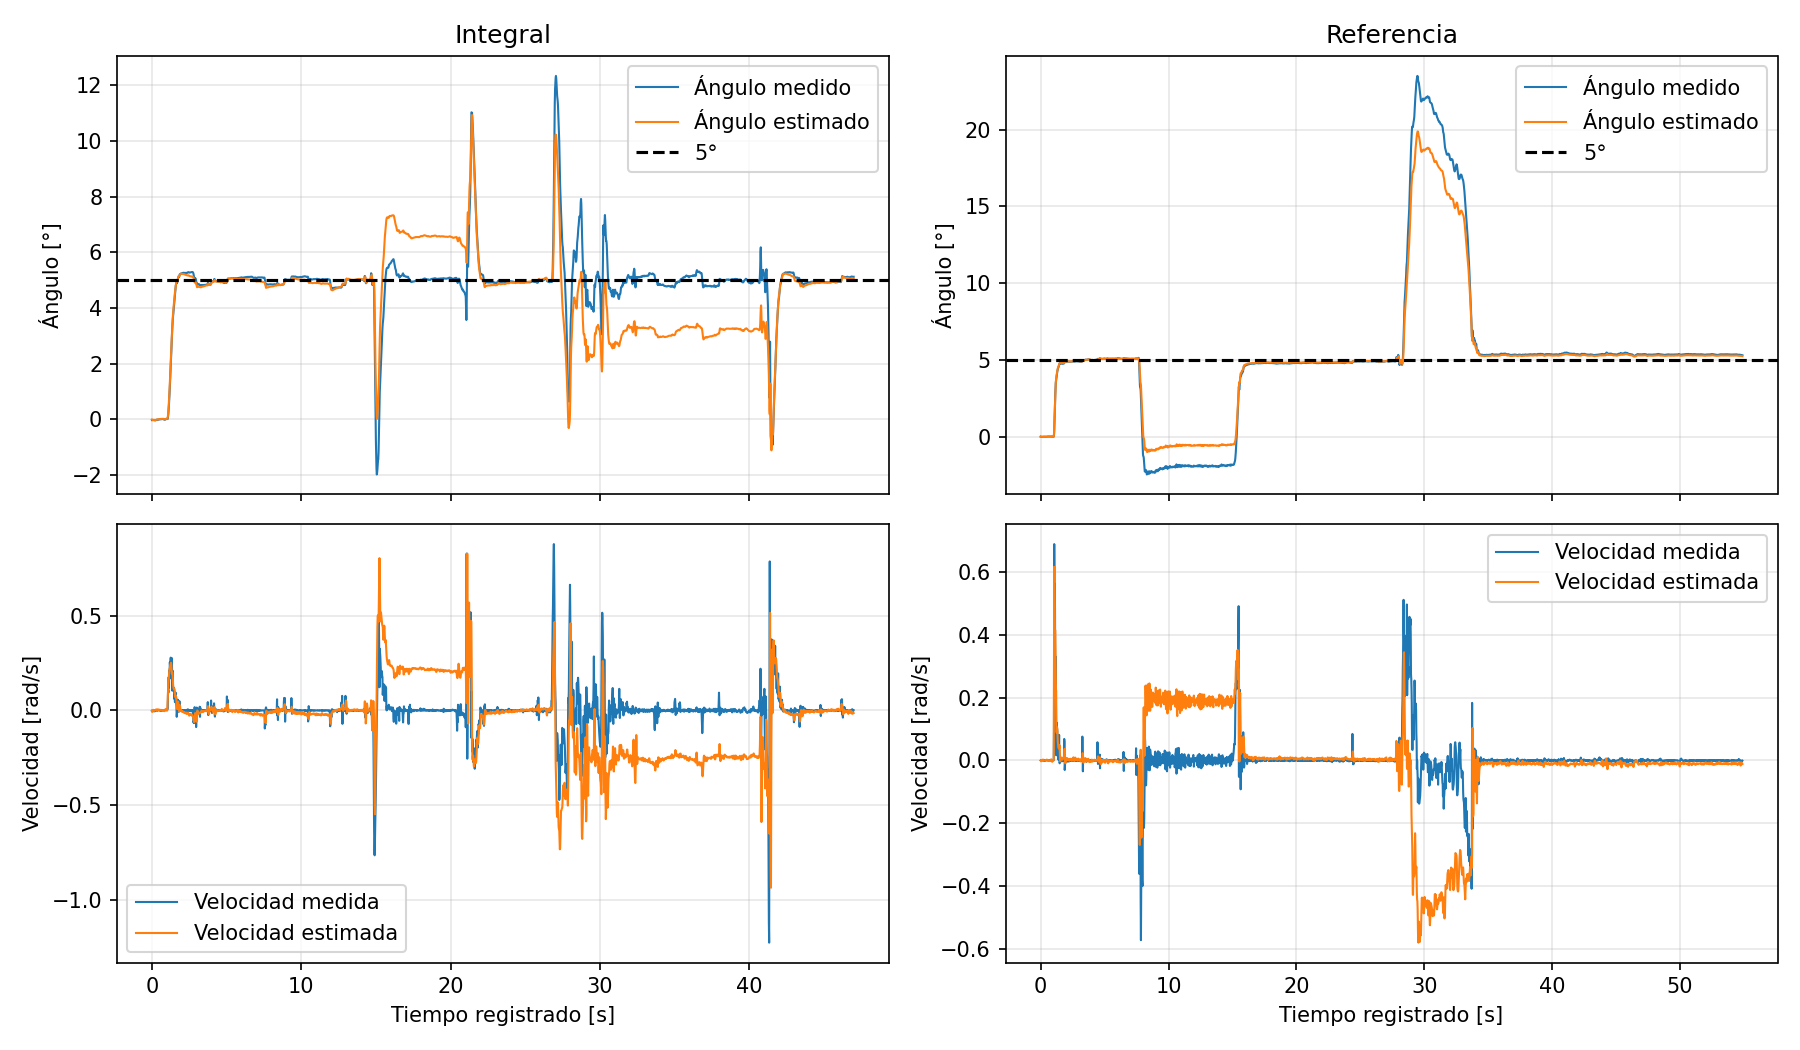
\includegraphics[width=\linewidth]{integral_vs_referencia.png}
\end{center}
{\small Azul: medición; naranja: estimación. La línea negra marca $5^\circ$.
Las columnas corresponden a ensayos distintos; los ejes verticales tienen
escalas diferentes.}

\textbf{Izquierda: con integrador.}
Tras las perturbaciones, el ángulo medido vuelve aproximadamente a $5^\circ$.
Entre unos 30 y 40 s, el observador estima cerca de $3{,}2^\circ$, pero la medición
queda cerca de $5^\circ$. La memoria $q$ permite compensar ese desacuerdo porque
acumula el error \emph{medido}. No hace falta que ambos ángulos coincidan para
que la medición siga la referencia.

\textbf{Derecha: con $F_r$.}
Primero llega a $5^\circ$. Entre unos 8 y 15 s, el ángulo medido queda cerca de
$-1{,}9^\circ$: el control no elimina ese desplazamiento mientras persisten esas
condiciones. Más adelante alcanza unos $23{,}5^\circ$ y termina cerca de
$5{,}36^\circ$. El registro muestra desplazamientos y errores finales; por sí solo
no demuestra una inestabilidad creciente.

\textbf{La pista del observador.}
Entre 10 y 15 s del ensayo con $F_r$, el giroscopio mide velocidad cercana a cero,
pero el observador estima alrededor de $+0{,}2\,\mathrm{rad/s}$.
Ese desacuerdo es compatible con una perturbación que el modelo no contempla;
no es solamente un retraso pasajero de la estimación.

\textbf{Qué podemos concluir.}
$F_r$ ajusta el seguimiento para el modelo nominal; el integrador agrega memoria
para compensar errores persistentes. Un empujón que se retira debería permitir
volver cerca de la referencia si el conjunto es estable y recupera las condiciones
originales. Cambiar y mantener el equilibrio es distinto: puede dejar error con
$F_r$. Como no registramos la orden al servo ni la perturbación aplicada, no
podemos confirmar saturación ni atribuir cada salto a una causa exacta.
Además, las ganancias $K$ son distintas: la comparación incluye ese cambio.

\subsection{Análisis Comparativo frente a Perturbaciones: Prealimentación ($F r$) vs. Estado Integrador ($H q$)}

\subsubsection{Limitaciones de la Prealimentación ($F r$) ante Perturbaciones No Modeladas}
La ley de control por prealimentación $u = -K\hat{x} + F r$ opera en lazo abierto con respecto al error de seguimiento instantáneo $e(t) = r(t) - y(t)$. La ganancia $F$ se calcula asumiendo un modelo nominal perfecto de la planta ($\dot{x} = A x + B u$). Ante la presencia de una perturbación física constante o un desplazamiento del punto de equilibrio mecánico (representado por un término externo $d$), la dinámica real del sistema se convierte en:
\begin{equation}
\dot{x}(t) = A x(t) + B u(t) + d
\end{equation}
Dado que el término $F r$ depende exclusivamente de la consigna de referencia $r$ y no monitorea la salida real $y(t)$, la acción de control no se adapta ante la presencia de $d$. Como consecuencia, el sistema se estabiliza en un punto de equilibrio desplazado, generando un error permanente en estado estacionario.

Asimismo, la perturbación no contemplada genera una discrepancia entre la medición del sensor $y(t)$ y la salida estimada por el observador de Luenberger $\hat{y}(t) = C\hat{x}(t)$. El término de corrección $L(y - C\hat{x})$ intenta compensar esta diferencia, pero al no estar modelada la fuente de la fuerza externa, distorsiona la estimación de las variables de estado internas (en particular, la velocidad angular $\hat{\omega}$), provocando respuestas erráticas en el actuador.

\subsubsection{Rechazo Automático de Perturbaciones mediante la Acción Integral ($H q$)}
A diferencia de la prealimentación, la incorporación del estado ampliado $q(t) = \int_{0}^{t} (r(\tau) - y(\tau)) \, d\tau$ establece un esquema de lazo cerrado directo sobre el error residual. La ley de control ampliada $u = -K\hat{x} + H q$ no requiere conocer a priori la magnitud ni el origen de la perturbación $d$.

Si una fuerza externa desvía la barra de la posición deseada ($y \neq r$), la variable acumuladora $q(t)$ integra dicha diferencia en cada período de muestreo. Al multiplicarse por la ganancia $H$, la señal enviada al actuador se incrementa progresivamente hasta alcanzar un valor en régimen permanente $u_{\text{ss}}$ que satisface la condición de equilibrio:
\begin{equation}
B u_{\text{ss}} + d = \mathbf{0}
\end{equation}
De esta forma, la acción integral genera de manera automática un torque de magnitud idéntica y sentido opuesto a la perturbación externa, cancelando su efecto y garantizando el restablecimiento del ángulo de la barra en la referencia $r$ con error nulo en estado estacionario.

\end{document}